\section{Further Research Trends}

This section is not intended to describe every aspect to its fullest, but to illustrate a showcase of possible and/or desirable developments of VR and HMD in the near future. 

Some mentioned technologies are only predictions and it is a matter of time to show which will become a reality in the next couple of years.

Predictions are to be on the leading edge which will be high end PC VR. These innovations will find its way into mobile VR over time, but the power, compute and pricing advantages will mean that computer generated virtual environments will provide the most sophisticated experience for a very long time.

\subsection{Improvements For VR Games}
\subsubsection{General Interaction}

Right now there are the following options available to receive input from a user in the virtual environment.
\begin{itemize}
	\item Physical controller
	\item Voice/sound recognition
	\item Body tracking
	\begin{itemize}
		\item Camera
		\item Infrared
		\item Ultrasound
	\end{itemize}
\end{itemize}

In future applications researchers have to find new interaction methods to receive input of the user. In many VR related companies this research is already starting or fully at it. 

Here are some examples for new interaction methods:

\begin{description}
	\item[SteamVR controller] New prototypes have a much smaller 'handprint' than what's in the hands of HTC Vive users today. The prototypes are not so much held as they are (optionally) gripped; a band hooking over the side of the user’s palm connects the core of the controller to a sort of backhand gripper which appears to keep the controller attached to the hand even while it isn’t being held.
	\item[Noitom Hi5 VR Glove~\textcopyright] The first wireless consumer glove designed for virtual reality headsets. You can now have both hands in the game thanks to our IMU sensor technology. 
\end{description}

\begin{figure}
	\centering
	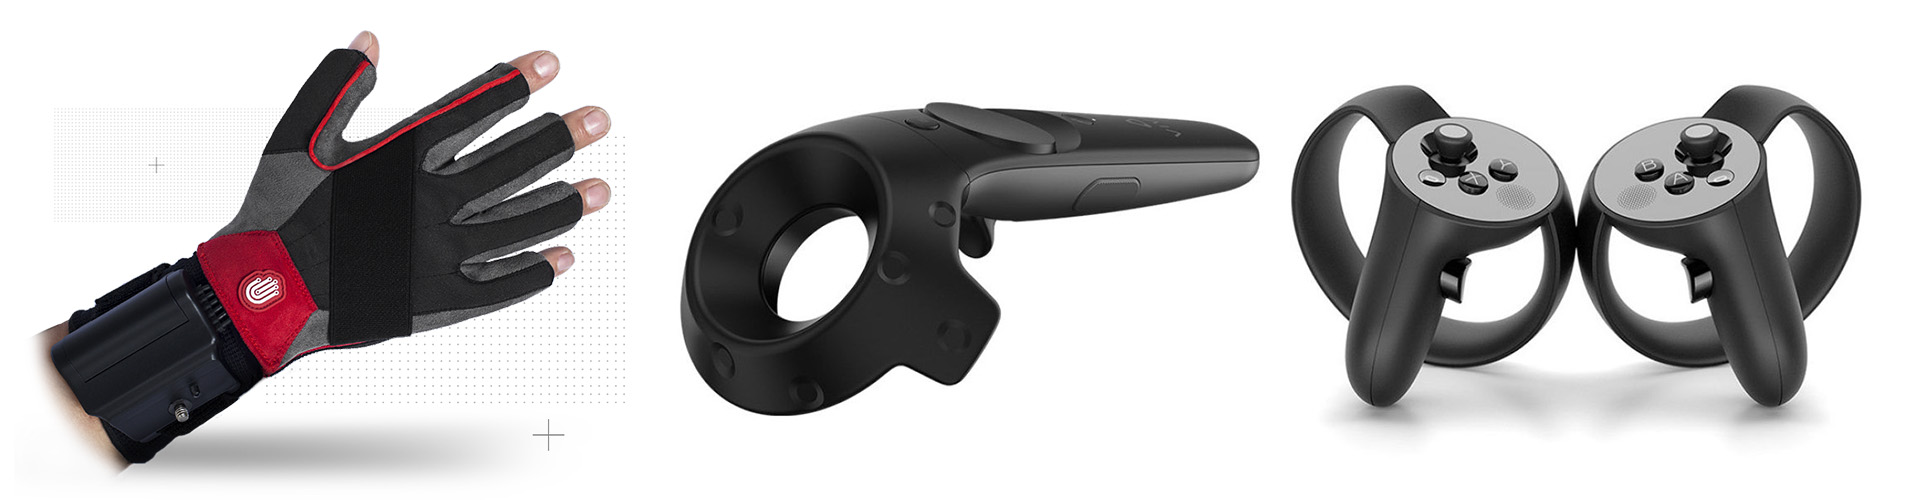
\includegraphics[width=0.99\columnwidth]{./figures/interaction}
	\caption[Game Controllers]{Different interaction methods for todays VR systems. FLTR: Hi5 VR Glove, HTV Vive Game Controller, Oculus Rift Game Controller~\footnotemark}~\label{fig:interaction}
\end{figure}
\footnotetext{\textcopyright~Noitom, Hi5 Vr Glove; roadtovr.com, VR motion controllers, [Online; accessed January 06., 2017],[Digitally revised] \url{http://hi5vrglove.com/images/hand1.png}, \url{http://www.roadtovr.com/wp-content/uploads/2016/07/vr-motion-controllers.jpg}}

\subsubsection{Locomotion}
\label{sec:locomotion}

\begin{figure}
	\centering
	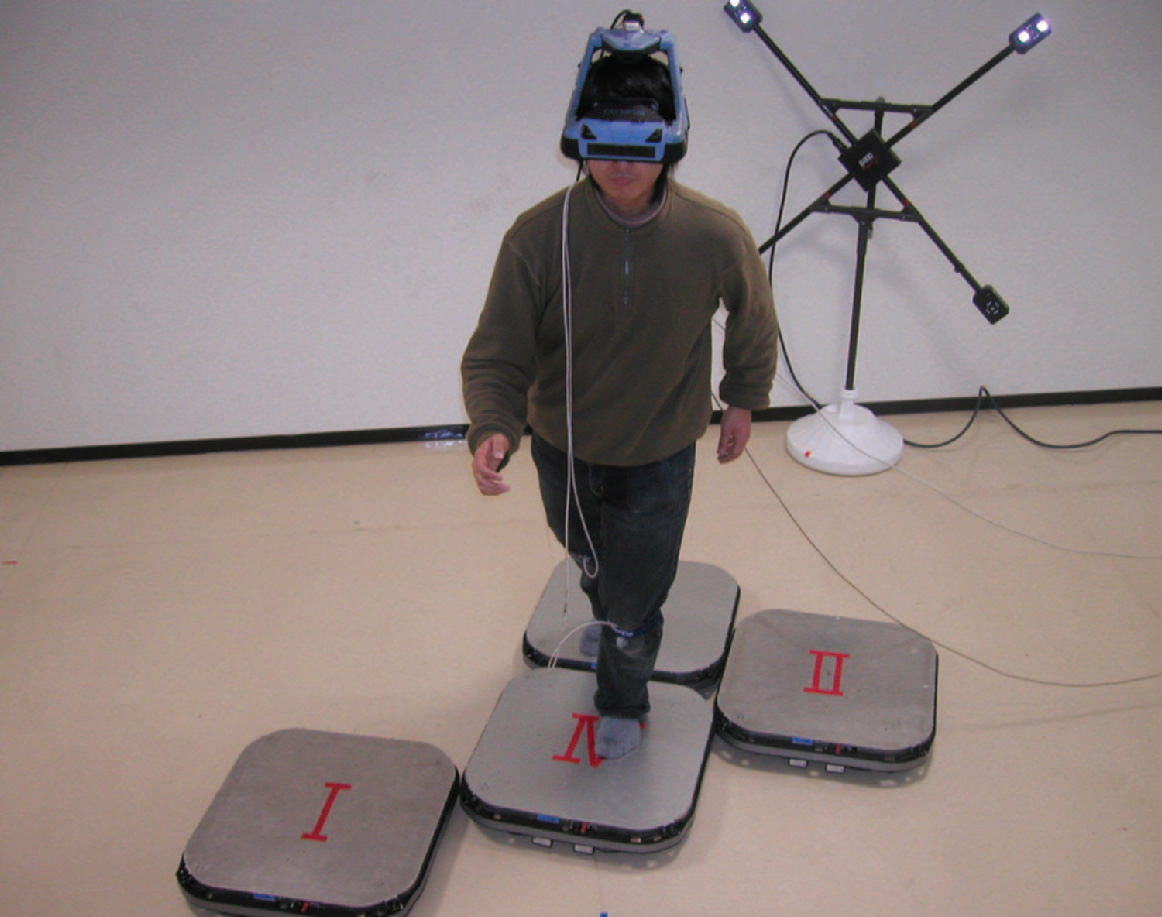
\includegraphics[width=0.99\columnwidth]{./figures/01381227}
	\caption{Overall view of CirculaFloor.}~\label{fig:cirFloor}
\end{figure}

\begin{description}
	\item[Point \& teleport locomotion] In this technique, users simply point where they want to be in virtual world and they are teleported to that position. As a major advantage, it is not expected to introduce motion sickness since it does not involve any visible translational motion. Advantages and possible alternatives are described in \textit{Point \& Teleport Locomotion Technique for Virtual Reality}~\cite{Bozgeyikli:2016:PTL:2967934.2968105}
	\item[Natural locomotion with actual transition] Approaches like the one taken by Hiroo Iwata, Hiroaki Yano, Hiroyuki Fukushima in their CirculaFloor~\cite{Iwata:2005:CLI:1078037.1079777} as seen in \textbf{Figure~\ref{fig:cirFloor}}. It was aimed to design a new hardware architecture that would be easy to upgrade the actuation mechanism or add new mechanisms for the creation of uneven surfaces. To achieve these goals, a configuration for a locomotion interface using a set of omnidirectional	movable tiles was designed. \newline Each tile is equipped with a holonomic mechanism that achieves omnidirectional motion. An infinite surface is simulated by the circulation of the movable tiles. Position sensors measure the motion of the feet. The tile moves in the opposite direction of the walker’s measured direction, canceling the motion of the step. This computer-controlled motion of the tiles fixes the walker’s position. The circulation of the tiles can cancel the walker’s displacement in an arbitrary direction. Thus, the walker can freely change direction while walking. 
	
	Another approach made by Souman et. al.~\cite{Souman:2010:MVW:1670671.1670675} shows the potential for omnidirectional treadmills. An algorithm was developed to steer the speed of a treadmill in such a way that VR immersiveness is not disrupted by changes in treadmill velocity. This algorithm was developed to work with an omnidirectional treadmill, allowing for changes in both walking speed and direction. A user can therefore walk in place and the VR system defines the world around him as endless space. This approach tackles problems better than the CirculaFloor because it generates less disturbance in the users walking.
	
	An omnidirectional treadmill is also being developed by \textit{Virtuix} with their \textit{Omni Gaming Treadmill~\textcopyright}. The Omni uses a concave, low-friction platform that enables a smooth gait and immersive walking and running motion. Omni shoes with a low-friction sole allow for comfortable, extended gameplay and a robust support ring and unattached support harness provide safety and versatility during rapid, unconstrained movements.
	
	A third approach has been made by the game developers of the game PORTAL. Building rooms completely out of tiles controlled by robotic arms can outline a whole room. Configurable, expendable and in moderate size. Combining this with VR holds great potential to create the perfect illusion. A schematic portrayal of this functionality can be seen in \textbf{Figure~\ref{fig:portallabrattest}}
	A imaginable application is when the tiles are intelligently configured to 'disappear' (into the ground) behind the player and appear in front of him kind of like a hamster wheel, making the playable area seem infinitely large to the player. The principle would be similar to the one described in CirculaFloor where the main disadvantage is that the floor tiles are unstable and not yet matured enough to provide sufficient support when walking at normal speed.
\end{description}

In games developed today often implemented are 'virtual walls' to keep people from walking into physical items like furniture, 
walls, stairs et cetera. It is interesting to notice that this is important because VR is not yet ready to support full shape recognition in the living room. With this the HMD could detect hazardous situations or items and the game could render it as something the user might not want to touch. The experience provided by this would be more seamless.
It is also important to implement shape recognition so that the users attention could be actively steered into direction that are open and save for the user to walk. On the downside the base station of the VR system must have an enormous amount of computational power to make these kind of calculations.

\begin{figure}
	\centering
	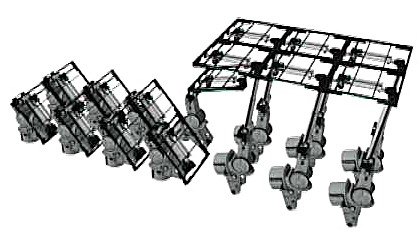
\includegraphics[width=0.99\columnwidth]{./figures/portallabrattest}
	\caption[Portal 2 : Lab Rat Panel Test]{Screenshot from the promotional video 'Portal 2 : Lab Rat Panel Test' (\ccbyncsa) of the game \textit{Portal 2 \textregistered\textcopyright} showing the general setup of floor panels mounted to robotic arms. This method enables developers to modify the structure of the floor at runtime.\footnotemark}~\label{fig:portallabrattest}
\end{figure}
\footnotetext{\textcopyright~Valve Software, Portal 2, [Online; accessed November 05., 2016],[Digitally revised] \url{https://www.youtube.com/watch?v=S7vFxs0ycn0}}

\subsubsection{Sight}

Head mounted displays of today have far less pixel density, a narrower field of view (FOV) and the lenses used have no actual method of actively focusing what the user is looking at.

To work on pixel density together with field of view has 2 approaches which accompanies an interesting trade-off in the usage of the resulting display resolution. Pixel density is a function of both, display resolution and field of view. One can have a higher pixel density image with a narrower field of view, or a wider field of view with a lower pixel density image. 

It all depends on what FOV is achievable and how compelling a wider FOV turns out to be.

A wider field of view with higher resolution will require a breakthrough in optics. Todays available lenses have a limited field of view without noticeable distortion, so new optics technology will be required.
The used lenses have also a fixed focus and while the human eye can adapt to different distances between objects the lenses of today stay focused around a distance of two meters.

The last point can be addressed with research field like \textit{holographic displays}, \textit{light field displays}, \textit{multifocal displays} or \textit{varifocal displays} and todays research teams are already on the subject.

The cumulative affect of depth of focus, higher resolution wider field of view and better optics will be VR that is highly comfortable, amazingly realistic and deeply convincing.

\subsubsection{Smell}

There are almost no studies what smell provides for virtual reality and this subject is hard do depict and predict. Over all smell provides a new dimension of immersion to a virtual environment and is after all one of the five basic senses of man, although negligible compared to visual and acoustic perceptions.

\subsubsection{Touch}

Using some similar technology to the iDummy\footnote{"IDummy" IDummy Product Website, 2015, accessed November 05., 2016, \url{http://www.idummy.com/}} by Chan et. al. one can create various objects of different size and shape. A user wearing a VR Headset can see a specific object and feel it as if it was the real thing. Using the technology developers can extend the realm of VR to one more dimension. Together with the technology~\cite{Azmandian:2016:HRD:2858036.2858226}

The iDummy is a mannequin technology where different body parts gan be modified by using multiple servo motors. The mannequin can change its chest circumference as well as hip measurement or the width of the waist to adapt to the needs of apparel designers and represent every body shape imaginable. 
By applying advanced mechatronics technology as the platform of mannequin development, Dr Allan Chan and his team members collected massive anthropometric data from worldwide population, as well as actual body scales from 3D Body Scanner, to create iDummy universal body scales and sizes. 

Adapting these principles to basic shapes, like cubes, balls or tetrahedrons a very haptic way of interacting with in game objects can be pursued. A user wearing a HMD can actually touch an object where the device in adding a visual abstraction. The player could with this method touch a ball of moderate size and see a basketball in the virtual representaion of this.

Comparable research has been done on shape changing interfaces, in example by Rasmussen et. al.~\cite{Rasmussen:2012:SIR:2207676.2207781}. They define 8 types of change for objects in 2 categories. 

\begin{description}
	\item[Topologically equivalent] Change of \textit{orientation}, \textit{form},  \textit{volume}, \textit{texture} \textit{viscosity} and \textit{spatiality}.
	\item[Not topologically equivalent] \textit{Addition or subtraction} and \textit{permeability} of materials.
\end{description}

With modifications to the object a person is holding often comes the impression of irreality if just minor features of this objects are not as expected by the person interacting. 
Psychologically the subject needs to be investigated since no proposition regarding divergent perception using HMD have been made.

Further Azmandian et. al. have already approached the topic of dynamic retargeting in their publication \textit{Haptic Retargeting: Dynamic Repurposing of Passive Haptics for Enhanced Virtual Reality Experiences}~\cite{Azmandian:2016:HRD:2858036.2858226}. The goal was to create a design space where game developers may reuse the physical objects in a person’s vicinity to provide a sense of touch when reaching, grabbing, lifting, or otherwise manipulating artifacts in a virtual reality scene, but to not be limited by what specific objects are around and whether they are located in the ''right'' place.

\subsubsection{Taste}
Similar to the sense of smell taste is a dimension of interaction not seen by many games. Virtual reality at this moment offers no way of tasting something seen in a virtual environment. This has also not been addressed in other applications but research has been made. There are times when a user might want to percept a taste and other times when we would hope not to do so, same goes for the smelling aspect of games at cetera.

Ranasinghe, Nimesha and Do, Ellen Yi-Luen~\cite{Ranasinghe:2016:VSS:2984751.2985729} have developed a way to address the taste buds using electrical stimulation. The proposed method is built on existing research that has highlighted the possibility of generating taste sensations by heating and cooling the human tongue. Right now they have only simulated sweet sensations as described in \textit{Virtual Sweet: Simulating Sweet Sensation Using Thermal	Stimulation on the Tip of the Tongue}. Other tastes would also be imaginable.

Unresolved remains the question of how this be included in the HMD? It would be impractical to attach a mask to the devices just to have taste and smell in a game.

\subsubsection{Hearing}

Research has to be done to best create head related transfer functions (HRTF). 

Humans can locate sounds in three dimensions – in approximate distance and direction. This is possible because the brain, inner ear and the external ears work together to make inferences about location.

HRTFs describe how audio has to be produced with a limited amount of audio sources to give the illusion that a sound is coming from a given point in space.

Continuing the research of the next decade has to tackle the problem of attention steering. Sound can be very helpful in getting a user to turn his head in one direction or to prevent him from bumping into objects located in the area he is playing a VR game. This can be helpful along with virtual walls, as described in the section \textit{Locomotion~\ref{sec:locomotion}} from above.

Sound propagation will be another aspect of research in the future where the virtual environment will become more convincing in its appearance. How sound reflects, diffracts and interferes with objects in VR is an important point for the future.

Sound can also be used to interact with VR devices.

For a convenient method of interaction with devices that do not use controllers by default such as the \textit{Samsung Gear VR} or \textit{Daydream View} Zayer, et. al. have developed the PAWdio~\cite{Zayer:2016:PHI:2967934.2968079}, a method to determine the general position of the users hand using acoustic sensing. It works by using properties of sound such as the Doppler effect to provide user input. Compared with vision based sensing it can be implemented with little computational overhead. 

Although some problems are given naturally by this method it provides a basic approach to take VR to every smartphone and with that to many more people than before.

\subsection{Health Aspects}

\begin{description}
	\item[Virtual reality sickness] \textit{(Also cybersickness)} Occurs when exposure to a virtual environment causes symptoms that are similar to motion sickness. \newline The most common symptoms are general discomfort, headache, stomach awareness, nausea, vomiting, pallor, sweating, fatigue, drowsiness, disorientation, and apathy. \newline Virtual reality sickness is different from motion sickness in that it can be caused by the visually-induced perception of self-motion; real self-motion is not needed.
\end{description}

Cybersickness has been discussed by Kay M. Stanney, Robert S. Kennedy and Julie M. Drexler back in 1997~\cite{stanney1997cybersickness}. Studying the symptoms and their effects on test subjects they found that users where experiencing cybersickness on different levels. In order to provide a context, he suggested that individuals who report symptoms which tally higher than 15 on the Simulator Sickness Questionnaire, would be experiencing sufficient discomfort that, unless there were other incentives, they would not voluntarily seek additional exposure because of the level of discomfort. 

It is found that cybersickness is a problem that must be corrected in order for virtual environments to be usable by anyone who wishes to use them~\cite{lo2001cybersickness}. So the important question arises as to how one can eliminate cybersickness or at least reduce its severity so people who are susceptible to cybersickness can use virtual environments.

It is a subject of investigation how health games can be beneficial for users. Virtual reality might not be the best purpose for games intended to increase the physical health of users, but until now no company has tackled the subject with medical support or professional health training advice. Other devices like the Wii fit with the balance board have shown that the demand for entertaining training is existent.
Using this HMD need to be a lot lighter than they are today. Also they have to be developed to be more ergonomic and comfortable to wear.

VR games could be used to help in the treatment of people with mental problems. Since VR is more immerse than 'normal' games it could be discovered that people suffering from asperger syndrome benefit from games in VR and head mounted devices.
Also VR game developers must research what is with people who suffer from anxiety disorders. It it important to know the downside of virtual environments and the immerse way that can sometimes evoke anxiety states from frightening situations experienced in games. A suggestion is that games offer different degrees of abstraction or alienation to differentiate between VR and the real world. The user can thereby choose the level of immersion himself.

\subsection{Increasing The Performance Of Devices For VR Gaming}

The last paragraph convoying this section is devoted to performance of the base station, consoles or mobile devices to deliver virtual environments to HMDs and offer a seamless and persuasive experience.

The question that has to be answered is: how can VR become wireless, more efficient and maybe leave a base station fully in the future?

Regarding wireless connections to the base station the first approaches towards a mobile experience have been made by HTC Corporation with the new technology named \textit{TP CAST for Vive}~\footnote{\textcopyright~HTC Corporation, TP Cast, 2016, accessed January 03., 2017 \url{https://www.vive.com/us/newsroom/2016/2016-11-11/}}

In November 2016 HTC has unveiled a breakthrough tether-less VR upgrade kit (preview edition) for VIVE VR system developed and produced by TPCAST, a Vive X Accelerator invested company. This 
kit will enable for the first time, users of high-end PC VR systems to have a fully untethered experience without compromising quality on all current Vive VR devices.
Advantages of this are the gained space opportunity and mobility within the gaming area.

Another question is why 90 frames per second are required by most VR games?

Too low of a frame rate in VR is probably one of the biggest causes of VR-sickness. The issue is with the refresh rate of the screen. When the frame rate is changing and/or not matching evenly with the refresh rate of the screen (90Hz in this case), the user gets perceived judder/tearing and all sorts of visual nastiness. On a standard monitor users can ignore this for the most part unless visuals matter a lot for them. But for VR, having a jerky uneven refresh of your display is all sorts of disorientating and generally quite uncomfortable.
